\id{МРНТИ 52.47.17}{}

\begin{articleheader}
\sectionwithauthors{Ж.К. Зайдемова, М.Д. Бисенгалиев, Ш.М. Медетов, Г.Ш. Досказиева, Г.Г. Абдешева, Г.Е. Суюнгариев, А.Н. Мукамбеткалиева}{ФИЛЬТРАЦИЯ НЕСЖИМАЕМОЙ ЖИДКОСТИ В ВЕРТИКАЛЬНОЙ СКВАЖИНЕ}

{\bfseries
Ж.К. Зайдемова\alink{https://orcid.org/0000-0002-6628-024X},
М.Д. Бисенгалиев\alink{https://orcid.org/0000-0002-4776-2251}\textsuperscript{\envelope },
Ш.М. Медетов\alink{https://orcid.org/0009-0002-0137-228X},
Г.Ш. Досказиева\alink{https://orcid.org/0000-0003-3459-0515},
Г.Г. Абдешева\alink{https://orcid.org/0000-0003-2783-4695},
Г.Е. Суюнгариев\alink{https://orcid.org/0000-0009-4850-4294},
А.Н. Мукамбеткалиева\alink{https://orcid.org/0000-0003-2236-0333}
}
\end{articleheader}

\begin{affiliation}
НАО Атырауский университет нефти и газа имени Сафи Утебаева, Атырау, Казахстан

\raggedright \textsuperscript{\envelope }Корреспондент-автор: maks\_bisengali@mail.ru
\end{affiliation}

Результаты исследования позволили изучить процессы в призабойная зона
скважины (ПЗС) и стволе скважины в режимах, характерных осложненным
условиям эксплуатации без учета фильтрации. Однако, эксплуатация таких
скважин для добычи нефти неразрывно связана с фильтрацией вытесняемой из
пласта водонефтяной смеси. Поэтому при таких осложнениях необходимо
также исследовать режим работы ПЗС в условиях фильтрации, т.е.
фильтрационные процессы как в естественном проявлении, так и с
применением специальных фильтров. В связи с этим, для конкретизации
эксплуатационных параметров процесса добычи нефти ШСНУ исследуем
гидродинамику процесса вытеснения нефти из пласта с учетом применения
устройств для фильтрации {[}1{]}.

В нефтепромысловой практике применяются скважинные фильтрационные
устройства, среди которых гравийный скважинный фильтр представляет собой
наиболее простую и дешевую конструкцию, доступную в условиях
промыслового ремонта {[}2{]}. Для его создания в открытую в продуктивном
пласте часть ствола скважины засыпают крупнозернистым материалом
(например, гравий) и для предотвращения выноса засыпки потоком нефти в
верхней части ствола у кровли пласта устанавливают пакер сетчатого типа.

Целью данной статьи является вывод уравнений для расчета
гидротехнических характеристик нефтедобывающей скважины с гравийным
фильтром и их решение. На этой основе обоснованы рабочие параметры
процесса фильтрации без учета и с учетом влияния на ПЗС погружения
плунжера штанговых скважинных насосных установок (ШСНУ).

Выбор такого метода борьбы с пескопроявлением связано с тем, что, в
отличие от фильтратов перфорационной конструкции {[}3,4{]}.

{\bfseries Ключевые слова\emph{:}} гидротехнические характеристика,
фильтрация жидкости, пескопроявление, нефтеотдача пласта, гравийный
фильтр, плунжерный насос.

\begin{articleheader}
{\bfseries ТІК ҰҢҒЫМАДА СЫҒЫЛМАЙТЫН СҰЙЫҚТЫҚТЫ СҮЗУ}

{\bfseries
Ж.К. Зайдемова,
М.Д. Бисенгалиев\textsuperscript{\envelope },
Ш.М. Медетов,
Г.Ш. Досказиева,
Г.Г. Абдешева,
Г.Е. Суюнгариев,
А.Н. Мукамбеткалиева
}
\end{articleheader}

\begin{affiliation}
«С.Өтебаев атындағы Атырау мұнай және газ университеті» КеАҚ, Атырау, Қазахстан,

e-mail: maks\_bisengali@mail.ru
\end{affiliation}

Зерттеулер қортындысы ұңғыманың түп маңы аймағында және ұңғыма
оқпанындағы сүзілуді ескермеген кездегі пайдаланудың күрделендірілген
жұмыс жағдайымен сипатталатын режимдердегі үрдістерді зерттеуге
мүмкіндік берді. Алайда, мұнай өндіруге арналған мұндай ұңғымаларды
пайдалану қабаттан ығыстырылып шығарылатын су-мұнай қоспасының
сүзілуімен үздіксіз байланысты. Сондықтан мұндай күрделі жағдайларда
сүзілу жағдайындағы ұңғыманың түп маңы аймағының жұмыс режимін зерттеу
қажет, яғни табиғи сүзілу кезіндегі және арнайы сүзгілерді қолдану
кезіндегі сүзілу үрдісін зерттеу керек. Осыған байланысты, штангалы
ұңғымалық сорап қондырғысының (ШҰСҚ) мұнай өндіру үрдісінің пайдалану
көрсеткіштерін нақтылау үшін сүзгілеу құрылғыларын қолдануды ескере
отырып, қабаттан мұнайдың ығыстырылу үрдісінің гидродинамикасын
зерттейміз {[}1{]}.

Мұнай кәсіпшілігінің тәжірибесінде ұңғымалық сүзгі құрылғылары
қолданылады, олардың ішінде қиыршық тасты ұңғыма сүзгісі кәсіпшілік
жөндеу жағдайларына мүмкіндік беретін қарапайым және арзан конструкция
түрінде болады {[}2{]}. Оны құрау үшін өнімді қабатта ұңғыманың
оқпанының бір бөлігін ірі бөлшекті материалмен (мысалы қиыршық тас)
көмеді және көмілген материалды мұнай ағызып кетпеу үшін оқпанның жоғары
бөлігіне қабат шетіне тор тәріздес пакер орнатады.

Бұл мақаланың мақсаты қиыршық тасты мұнай өндіруші ұңғымалардың
гидротехникалық сипаттамаларын есептеуге арналған теңдеуді шығару және
оларды есептеу. Осы негізде штангалы ұңғымалық сорап қондырғысының ШҰСҚ
плунжерінің батуының ұңғыманың түп маңы аймағына әсер етуін ескерген
және ескермеген кездегі сүзілу үрдісінің жұмыстық көрсеткіштерін
негізделген {[}3,4{]}.

Құм көрінісімен күрестің осындай әдісін таңдау перфорациялық
конструкциялы сүзгіштерге қарағанда бірқатар артықшылықтарға ие болуымен
байланысты түсіндіріледі.

{\bfseries Түйін сөздер:} гидротехникалық сипаттама, сұйықтың сүзілуі, құм
көрінісі, қабаттың мұнай бергіштігі, қйыршық тасты сүзгі, плунжерлі
сорап.

\begin{articleheader}
{\bfseries FILTRATION OF INCOMPRESSIBLE FLUID IN A VERTICAL WELL}

{\bfseries
Zh.K. Zaidemova,
M.D. Bisengaliev\textsuperscript{\envelope },
Sh.M. Medetov,
G.Sh. Doskazieva,
G.G. Abdeshova,
G.E. Suyungariyev,
A.N. Mukambetkalieva
}
\end{articleheader}

\begin{affiliation}
NAO Atyrau University of Oil and Gas named after Safi Utebaev, Atyrau, Kazakhstan

e-mail: maks\_bisengali@mail.ru
\end{affiliation}

The results of the research allowed to study the processes in
bottom-hole zone (BHZ) and wellbore in the regimes characteristic of
complicated operating conditions without taking into account filtration.
However, the operation of such wells for oil production is inextricably
linked with filtration of water-oil mixture displaced from the
reservoir. Therefore, under such complications it is also necessary to
investigate the operation mode of the CCD under filtration conditions,
i.e. filtration processes both in natural manifestation and with the use
of special filters. In this connection, for specification of operational
parameters of the process of oil production by SHSNU we study the
hydrodynamics of the process of oil displacement from the reservoir
taking into account the application of filtration devices {[}1{]}.

In oilfield practice, downhole filtration devices are used, among which
gravel downhole filter is the simplest and cheapest design available in
the conditions of field repair {[}2{]}. To create it, a coarse-grained
material (e.g., gravel) is poured into the open part of the wellbore in
the productive formation and a net-type packer is installed in the upper
part of the wellbore near the formation roof to prevent the oil flow
from carrying the filling away.

The purpose of this article is to derive equations for calculating the
hydraulic characteristics of an oil production well with a gravel filter
and their solution. On this basis, justification of the operating
parameters of the filtration process without taking into account and
taking into account the effect on the CCD of plunger immersion of rod
well pumping units (RWPU). The choice of such a method of struggle
against sand penetration is connected with the fact that unlike
perforation design filtrates {[}3,4{]}.

{\bfseries Keywords:} hydraulic engineering characteristics, fluid
filtration, sanding, oil recovery, gravel filter, plunger pump.

\begin{multicols}{2}
{\bfseries Введение.} Из общего объема ежегодно добываемой в республике
нефти более чем 80\% приходится месторождениям, находящимся на последней
стадий эксплуатации. В связи с этим, не смотря на интенсивное освоение
новых нефтяных месторождений Казахстана, проблема повышения
эффективности эксплуатации, в частности интенсификации нефтеотдачи
пластов существующих месторождений и увеличения их межремонтного периода
все еще остается важной научно -- производственной проблемой.

Решение таких задач, прежде всего, связано с применением комплекса
научно обоснованных мероприятий, направленных на совершенствование
рабочих процессов, методов и технических средств воздействия на пласт,
способствующих интенсификации и снижению себестоимости добычи нефти. При
многочисленности существующих способов и методов воздействия на пласт,
вопрос о научном обосновании их оптимального выбора в каждом конкретном
случае эксплуатации скважин, с учетом влияния на дебит рабочих
параметров применяемых технических средств добычи представляет собой
огромный научно-практический интерес.

Если учесть, что 70\% действующего фонда скважин старых нефтяных
месторождений, эксплуатируемых как в республике, так и в ближнем
зарубежье осваиваются при помощи ШСНУ, то станет очевидным, какое
влияние может оказать на нефтеотдачу оптимальный выбор режима их работы,
совершенствование уравновешивания привода при рациональном сочетании с
тем или иным способом воздействия на пласт. Такой подход решения
вышеуказанной задачи путем комплексного рассмотрения вопросов
уравновешивания привода и колебания подземной части ШСНУ с учетом
влияния различных динамических факторов предопределяет повышение дебита
скважин и получение более достоверных результатов исследований.

В связи с этим, исследования направленные на изучение влияния на дебит
скважин упругого уравновешивания привода плунжерных насосов и
оптимизация способов воздействия на пласт в условиях пескопроявления
являются актуальными.

{\bfseries Материалы и методы.} Фильтрацию несжимаемой жидкости (нефти) в
вертикальной центральной скважине, эксплуатирующей горизонтальный пласт
толщиной \emph{в} (рисунок 1). Поток жидкости внутри ствола скважины
примем за одномерный, направленный вдоль оси $z$, т.е. радиальной
составляющей течения внутри ствола скважины. Неравномерностью потока по
ее сечению пренебрегаем. Поэтому вертикальную составляющую $u(z)$
скорости течения будем считать зависящей только от одной координаты
$z$. Приведенное давление {[}5{]}.

\begin{equation}
P^{(t)}=\rho gz+p+\rho\left(\frac{V_1^2}{2}-\frac{V_2^2}{2}\right),
\end{equation}

где $\rho$ -- гидродинамическое давление; $\rho$ -- плотность
флюида; $g$ -- ускорение свободного падения; $z$ --
координата, направленная вертикально вверх по оси скважины, начало
отсчета на которой совмещено с подошвой пласта (рисунок 1), внутри
скважины в первом приближении тоже считаем функцией только лишь
координаты $z$.

Связь между скоростью $u(z)$ и давлением $Р$ определяется из
закона фильтрации для фильтра скважины

\begin{equation}
\frac{dP}{dz}=-f(u),
\end{equation}

где 
-- заданная функция удовлетворяющая условию $f(0)=0$. В частности,
если в фильтре скважины фильтрация линейная, то

\begin{equation}
f(u)=\frac{\mu u}{k_2}.
\end{equation}

Если в фильтре режим фильтрации подчиняется двучленному закону, то

\begin{equation}
f(u)=Au+Bu^2,
\end{equation}

где $А$ и $B$ -- некоторые экспериментально устанавливаемые
положительные постоянные. Кроме перечисленных (3), (4) под $f$
$(u)$ могут пониматься и другие законы фильтрации, например
степенные.

{\bfseries Результаты и обсуждение.} Если функция $Р(z)$ будет
найдена, то с помощью (2) можно определить скорость $u(z)$,
а следовательно и дебит скважины $Q=\pi\cdot r_c^2\cdot u(b)$. Для
вывода уравнения, которому должна удовлетворять функция \emph{Р}
(\emph{z}), рассмотрим течение в скважине между двумя бесконечно
близкими плоскостями $z$ и $z+dz$ (рисунок 1) {[}6{]}. Течение
жидкости между плоскостями $z$ и $z+dz$ в первом приближении
будем рассматривать как плоскорадиальное. Поэтому величину притока
$dq(z)$ жидкости в части боковой поверхности ствола
скважины, заключенной между $z$ и $z+dz$, найдем по
известной {[}6{]} формуле Дюпюи:

\begin{equation}
dq(z)=\frac{2\pi k_1\cdot(P_{\text{П}}-P(z))\cdot dz}{\mu\cdot \ln\left(\frac{R}{r_c}\right)},
\end{equation}

где $P_{\text{П}}$ -- давление на контуре питания \\$r=R; P(z)$ --
давление в скважине. К величине $dq(z)$ добавляется поток
со стороны поступающей снизу жидкости, равный $\pi\cdot r_c^2\cdot
u(z)$ (рисунок 1). Поэтому за единицу времени в участок скважины
$[z,z+dz]$ поступает суммарный поток жидкости, равный $dq(z)+\pi\cdot r_c^2\cdot u(z)$.
\end{multicols}

\begin{figure}[H]
	\centering
	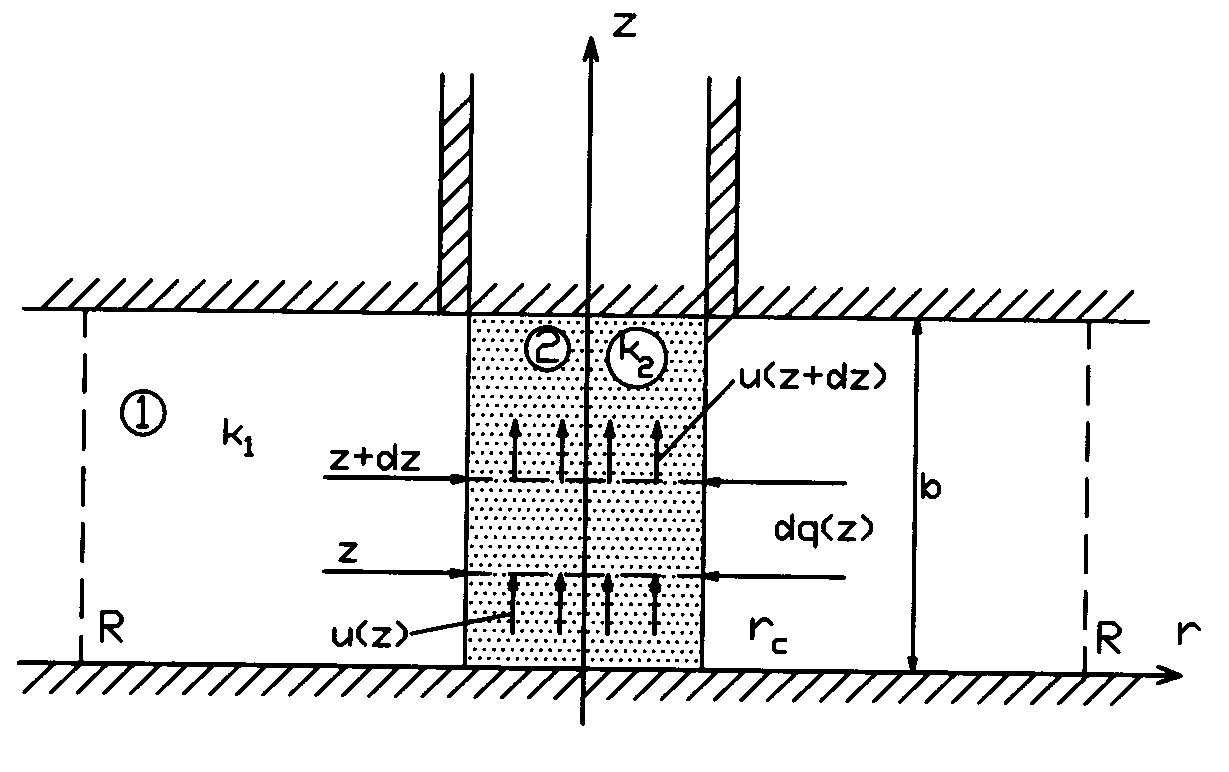
\includegraphics[width=0.7\textwidth]{media/gorn/image17}
	\caption*{\normalfont\emph{1 -- призабойная зона скважины (ПЗС) с проницаемостью
k\textsubscript{1} -- режим фильтрации линейный; 2 -- гравийный фильтр
(часть ствола скважины с засыпкой) -- режим фильтрации может быть (в
зависимости от его свойств) как линейным, так и нелинейным;
r\textsubscript{с} -- радиус скважины, k\textsubscript{2} -- коэффициент
проницаемости фильтра, r и z -- цилиндрические координаты, ось z
направлена вверх; R -- радиус контура питания; u(z) -- скорость течения
жидкости в фильтре скважины}}
	\caption*{Рис.1 -- Схема устройства гравийного скважинного фильтра и принятая модель течения жидкости в нем}
\end{figure}

Следовательно, в сечении скважины $(z+dz)$ вертикальная
составляющая скорости потока будет равна

\begin{equation}
u(z+dz)=\frac{dq(z)+\pi r_c^2\cdot u(z)}{\pi r_c^2}=u(z)+\frac{2k_1\cdot (P_{\text{П}}-P(z))\cdot dz}{\mu\cdot r_c^2\cdot \ln\left(\frac{R}{r_c}\right)}.
\end{equation}

С другой стороны, величина скорости $u\cdot(z+dz)$ связана с
распределением давления в стволе скважины по закону (2). Поэтому должно
быть выполнено равенство:

\begin{equation}
\frac{dP(z+dz)}{dz}=-f[u(z+dz)].
\end{equation}

Вычитая из (7) соответствующие части равенства (2), получим

\begin{equation}
\frac{dP(z+dz)}{dz}-\frac{dP(z)}{dz}=-\{f[u(z+dz)]-f[u(z)]\}.
\end{equation}

Если теперь к обеим частям последнего выражения применить известную в
математическом анализе теорему Лагранжа и перейти к пределу при
$dz$, то из (8) с учетом равенства (6) получим:

\begin{equation}
\frac{d^2P(z)}{dz^2}=-\frac{2k_1\cdot[P_{\text{П}}-P(z)]}{\mu\cdot r_c^2\cdot \ln\left(\frac{R}{r_c}\right)}\cdot f'[u(z)].
\end{equation}

Уравнение (9) содержит две неизвестные функции: приведенное давление
внутри ствола скважины $Р(z)$ и скорость потока жидкости в стволе
скважины $u(z)$. Поэтому для решения задачи еще нужно определить
уравнение для $u(z)$. Чтобы найти $u(z)$ воспользуемся
формулой (5) за весь приток жидкости к скважине на участке $[0,Z]$:

\begin{equation}
q(z)=\int_0^z dq(z)=\frac{2\pi k_1}{\mu\cdot\ln\left(\frac{R}{r_c}\right)}\cdot\int_0^z(P_{\text{П}}-P(z))dz.
\end{equation}

\begin{multicols}{2}
С учетом, что через сечение $z$ скважины должен проходить за
единицу времени поток жидкости $q(z)$, средняя скорость течения
жидкости $u(z)$ будет равна $\frac{q(z)}{\pi r_c^2},$ т.е.

\begin{equation}
u(z)=\frac{2k_1}{\mu\cdot r_c^2\cdot\ln\left(\frac{R}{r_c}\right)}\cdot\int_0^z(P_{\text{П}}-P(z))dz.
\end{equation}

Подставив (11) в (9), относительно неизвестной функции распределения
давления
в
стволе скважины получим одно интегро-дифференциальное уравнение. Для
решения этого уравнения нужно еще дополнительно задать краевые условия
на границах $z=0$ и $z=b$ активного участка скважины. В
сечении на кровле пласта $z=b$ (рисунок 1) должно быть задано
давление в скважине, поэтому

\begin{equation}
P|_{z=b}=P_C.
\end{equation}

В сечении $z=0$ (на подошве пласта) нормальная составляющая
скорости потока $u(0)=0$, а следовательно,

\begin{equation*}
\frac{dP}{dz}|_{z=0}=-f[u(0)]=-f(0)=0.
\end{equation*}

Поэтому

\begin{equation}
\frac{dP}{dz}|_{z=0}=0.
\end{equation}

{\bfseries Выводы.} Таким образом, интегро-дифферен\-циальное уравнение,
получающееся при подставке (11) в (9), должно интегрироваться совместно
с краевыми условиями (12) и (13).

После того, как функция $P(z)$ будет найдена, дебит $Q$ скважины
можно вычислить по формуле (10) при $z=b$:

\begin{equation}
Q=\frac{2\pi k_1}{\mu\cdot\ln\left(\frac{R}{r_c}\right)}\cdot\int_0^b(P_{\text{П}}-P(z))dz.
\end{equation}

Если вдоль ствола скважины давление $P(z)$ можно принять постоянным,
равным $P_c$, то из формулы (14) получается классическая формула Дюпюи
для дебита $Q_0$ центральной совершенной скважины

\begin{equation}
Q_0=\frac{2\pi k_1\cdot (P_{\text{П}}-P_C)\cdot b}{\mu\cdot\ln\left(\frac{R}{r_c}\right)}.
\end{equation}

Более простой по сравнению с (9), (11) и удачно его дополняющий способ
расчета гидротехнических характеристик скважины можно получить, если за
основу взять распределение скорости течения $u(z)$ в ее фильтре.
Поэтому в дополнение к (9), (11) выведем еще дифференциальное уравнение
для скорости фильтрации $u(z)$ {[}7 - 9{]}.

Прежде всего заметим, что для производной $\frac{du}{dz}$ из формулы
(6) с учетом (15) получается значение

\begin{equation}
\frac{du}{dz}=\frac{Q_0}{\pi\cdot r_c^2\cdot b}\cdot\frac{P_{\text{П}}-P(z)}{P_{\text{П}}-P_C}
\end{equation}

Дифференцируя обе части (16) по $z$ и учитывая формулы (2) и (15),
для скорости фильтрации $u(z)$ получим уравнение

\begin{equation}
\frac{d^2u}{dz^2}=\frac{Q_0}{\pi\cdot r_c^2\cdot b\cdot(P_{\text{П}}-P_C)}\cdot f(u)
\end{equation}

Дифференциальное уравнение (17) должно интегрироваться совместно с
краевыми условиями

\begin{equation}
u|_{z=0}=0\text{ и }\frac{du}{dz}|_{z=b}=\frac{Q_0}{\pi\cdot r_c^2\cdot b}.
\end{equation}

Первое из условий (18) означает, что нормальная составляющая скорости
потока на подошве пласта отсутствует, а второе условие сразу следует из
(16) при $z=b$.

Интегрирование уравнения (17) совместно с условиями (18) приводит к
следующему распределению скорости $u(z)$:

\begin{equation}
z=\frac{1}{A}\cdot\int_0^u\frac{du}{\sqrt{1-\frac{2}{A\cdot(P_{\text{П}}-P_C)}\cdot\int_u^{u_*}f(u)du}},
\end{equation}

где введены обозначения

\begin{equation}
A=\frac{Q_0}{\pi\cdot r_c^2\cdot b};\quad u_*=\frac{Q}{\pi\cdot r_c^2}=u(b).
\end{equation}

Уравнение для неизвестной постоянной $u_*$ получим с
помощью (19) при $z=b$. Учитывая (20), приходим к следующему
уравнению для $u_*$:

\begin{equation}
A\cdot b=\frac{1}{A}\cdot\int_0^{u_*}\frac{du}{\sqrt{1-\frac{2}{A\cdot(P_{\text{П}}-P_C)}\cdot\int_u^{u_*}f(u)du}}.
\end{equation}

Из уравнения (21) вычислим \emph{u}\textsubscript{*}, а стало быть и
дебит \emph{Q} по формуле (20). Затем по формуле (19) можно будет найти
распределение скорости \emph{u(z)} в фильтре скважины {[}10{]}. Наконец,
с помощью формул (16) и (19) найдем распределение давления в стволе
скважины по ее высоте:

\begin{equation}
\frac{P_{\text{П}}-P(z)}{P_{\text{П}}-P_C}\sqrt{1-\frac{2}{A\cdot(P_{\text{П}}-P_C)}\cdot\int_u^{u_*}f(u)du}
\end{equation}

Таким образом, задачу расчета гидротехнических характеристик скважины с
гравийным фильтром оказалось можно считать решенной. Это дает основание
анализировать работу фильтра для любого режима эксплуатации, в нашем
случае, для линейного режима.
\end{multicols}

\begin{center}
{\bfseries Литература}
\end{center}

\begin{references}
1. Зайдемова Ж.К., Ахметов С.М. Исследование процесса движения жидкости в
призабойной зоне и в стволе нефтегазодобывающей скважины в условиях
повышенного обводнения и пескопроявления // Сборник трудов Третьего
международного семинара -- совещания «Инновационные подходы в развитии
нефтегазовой и нефтехимической промышленности в Атырауской области».
-Атырау: АИНГ, 2005. -- С.345--358.

2. Пашкин~В.Д., Лежнев~К.Э., Кудря~Е.Р., Никулин~К.А. Гравийные фильтры
как средство контроля притока при разработке слабоконсолидированных
пластов.~PROНЕФТЬ. Профессионально о нефти.2022;7(1):52-59.~

3. Попов М.А., Петраков Д.Г. Исследование режимов эксплуатации газовых
скважин в осложненных условиях. Санкт-Петербургский горный университет.
Недропользование.2021. Т.21, № 1. С.36-41.

4. Шиян С.~И., Шаблий И.~И, Задачин А.~А., Сафиуллина Е.~У, Кусова Л.~Г
Перспективы применения методов повышения нефтеотдачи пластов на Полярном
нефтяном месторождении на основе анализа эффективности применяемых
методов на месторождениях-аналогах. // Нефтепромысловое дело. -- 2022.
-- № 3 (639). -- С.9--18.

5. Бисенгалиев М.Д., Абдешова Г.К., Досказиева Г.Ш. Конструкция
усовершенствованного цепного привода штанговой скважинной насосной
установки, «Нефть и газ» 2, 2025 год, 274-281 стр.

6. Зайдемова Ж.К., Ахметов С.М., Суюнгариев Г.Е. Перспективы
уравновешивания наземных приводов скважинных насосных установок
пружинными выравнивателями нагрузок //Доклады Первых международных
научных Надировских чтений «Научно-технологическое развитие
нефтегазового комплекса». - Атырау.-2003. - С.268 -271.

7. Шишкин Г.~А.~, Линейные интегро-дифференциальные уравнения
Фредгольма. Учебное пособие по спецкурсу и спецсеминару. Издательство
Бурятского госуниверситета 2007.-195 c.

8. Власов В. В., Перез Ортиз Р. Спектральный анализ
интегро-дифференциальных уравнений, возникающих в теории вязкоупругости
и теплофизике // Матем. Заметки.- 2015.-Т.98(4).- С.630-634
DOI https://doi.org/10.4213/mzm10829

9. Пулькина Л. С. Нелокальная задача для гиперболического уравнения с
интегральными условиями I рода с ядрами, зависящими от времени//Изв.
вузов. Матем.-, 2012.- №10.- С.32-34
DOI\\\href{https://doi.org/10.3103/S1066369X12100039}{10.3103/S1066369X12100039}

10. Сабитова Ю. К. Краевая задача с нелокальным интегральным условием
для уравнений смешанного типа с вырождением на переходной линии// Матем.
Заметки.- 2015.-Т.98(3). С.393-406. DOI 10.4213/mzm9135
\end{references}

\begin{center}
{\bfseries References}
\end{center}

\begin{references}
1. Zajdemova Zh.K., Ahmetov S.M. Issledovanie processa dvizhenija
zhidkosti v prizabojnoj zone i v stvole neftegazodobyvajushhej skvazhiny
v uslovijah povyshennogo obvodnenija i peskoprojavlenija // Sbornik
trudov Tret' ego mezhdunarodnogo seminara -- soveshhanija
«Innovacionnye podhody v razvitii neftegazovoj i neftehimicheskoj
promyshlennosti v Atyrauskoj oblasti». -Atyrau: AING, 2005. -- S.
345--358.{[}in Russian{]}

2. Pashkin V.D., Lezhnev K.Je., Kudrja E.R., Nikulin K.A. Gravijnye
fil' try kak sredstvo kontrolja pritoka pri razrabotke
slabokonsolidirovannyh plastov. PRONEFT''.
Professional' no o nefti.2022;7(1):52-59. {[}in
Russian{]}

3. Popov M.A., Petrakov D.G. Issledovanie rezhimov jekspluatacii gazovyh
skvazhin v oslozhnennyh uslovijah. Sankt-Peterburgskij gornyj
universitet. Nedropol' zovanie.2021. T.21, № 1.
S.36-41. {[}in Russian{]}

4. Shijan S. I., Shablij I. I, Zadachin A. A., Safiullina E. U, Kusova
L. G Perspektivy primenenija metodov povyshenija nefteotdachi plastov na
Poljarnom neftjanom mestorozhdenii na osnove analiza jeffektivnosti
primenjaemyh metodov na mestorozhdenijah-analogah. // Neftepromyslovoe
delo. -- 2022. -- № 3 (639). -- S.9--18{[}in Russian{]}.

5. Bisengaliev M.D., Abdeshova G.K., Doskazieva G.Sh. Konstrukcija
usovershenstvovannogo cepnogo privoda shtangovoj skvazhinnoj nasosnoj
ustanovki, «Neft'{} i gaz» 2, 2025 god, 274-281 str.
{[}in Russian{]}

6. Zajdemova Zh.K., Ahmetov S.M., Sujungariev G.E. Perspektivy
uravnoveshivanija nazemnyh privodov skvazhinnyh nasosnyh ustanovok
pruzhinnymi vyravnivateljami nagruzok //Doklady Pervyh \\mezhdunarodnyh
nauchnyh Nadirovskih chtenij «Nauchno-tehnologicheskoe razvitie
neftegazovogo \\kompleksa». - Atyrau.-2003. - S.268 -271. {[}in
Russian{]}

7. Shishkin G. A. , Linejnye integro-differencial' nye
uravnenija Fredgol' ma. Uchebnoe posobie po \\speckursu i
specseminaru. Izdatel' stvo Burjatskogo gosuniversiteta
2007. -195 c. {[}in Russian{]}

8. Vlasov V. V., Perez Ortiz R. Spektral' nyj analiz
integro-differencial' nyh uravnenij, voznikajushhih v
teorii vjazkouprugosti i teplofizike // Matem. Zametki.- 2015.-T.98(4).-
S.630-634 DOI \\10.4213/mzm10829. {[}in Russian{]}

9. Pul' kina L. S. Nelokal' naja zadacha
dlja giperbolicheskogo uravnenija s integral' nymi
uslovijami I roda s jadrami, zavisjashhimi ot vremeni//Izv. vuzov.
Matem.-, 2012.- №10.- S.32-34 DOI \\10.3103/S1066369X12100039. {[}in
Russian{]}

10. Sabitova Ju. K. Kraevaja zadacha s nelokal' nym
integral' nym usloviem dlja uravnenij smeshannogo tipa s
vyrozhdeniem na perehodnoj linii// Matem. Zametki.- 2015.-T.98(3). S.
393-406. DOI \\10.4213/mzm9135. {[}in Russian{]}
\end{references}

\begin{authorinfo}
\emph{{\bfseries Сведения об авторах}}

Ж.К. - , НАО
Атырауский университет нефти и газа имени С. Утебаева, Атырау,
Казахстан, e-mail: \href{mailto:b.n.m.99@list.ru}{\nolinkurl{b.n.m.99@list.ru}};

Бисенгалиев М.Д. -  ассоциированный
, НАО Атырауский университет нефти и газа имени С.
Утебаева, Атырау, Казахстан, e-mail: \href{mailto:maks\_bisengali@mail.ru}{\nolinkurl{maks\_bisengali@mail.ru}};

Медетов Ш.М. -  ассоциированный
, НАО Атырауский университет нефти и газа имени С.
Утебаева, Атырау, Казахстан, e-mail: \href{mailto:medetov.76@mail.ru}{\nolinkurl{medetov.76@mail.ru}};

Досказиева Г.Ш.- , НАО
Атырауский университет нефти и газа имени С. Утебаева, Атырау,
Казахстан, e-mail: \\doskaziyeva.gulsin@gmail.com;

Абдешова Г.Г.- ст преподаватель, НАО Атырауский университет нефти и газа
имени Сафи Утебаева, Атырау, Казахстан, e-mail: gulya6320@mail.ru;

Суюнгариев Г.Е. -  ассистент профессора,
НАО Атырауский университет нефти и газа имени С.Утебаева, Атырау,
Казахстан, e-mail: S.gabit72@mail.ru;

Мукамбеткалиева А.Н. - докторант, НАО Атырауский университет нефти и
газа имени С. Утебаева, Атырау, Казахстан, e-mail: ainash\_m\_89@mail.ru;

\emph{{\bfseries Information about the authors}}

Zaidemova Zh. - Ph. Sci, Professor, Atyrau Uni󠀁versity of Oil and Gas
nam󠀁ed aft󠀁er S. Ute󠀁baev, Aty󠀁rau, Kaz󠀁akhstan, e-mail:
b.n.m.99@list.ru;

Bissengaliyev M. -- Ph. sci, associate professor, Atyrau Uni󠀁versity of
Oil and Gas nam󠀁ed aft󠀁er S. Ute󠀁baev, Aty󠀁rau, Kaz󠀁akhstan, e-mail:
maks\_bisengali@mail.ru;

Medetov Sh. - Ph. Sci, Associate Professor, Atyrau Uni󠀁versity of Oil and
Gas nam󠀁ed aft󠀁er S. Ute󠀁baev, Aty󠀁rau, Kaz󠀁akhstan, e-mail: medetov.76@mail.ru;

Doskazieva G- Ph. Sci, Professor, Atyrau Uni󠀁versity of Oil and Gas nam󠀁ed
aft󠀁er S. Ute󠀁baev, Aty󠀁rau, Kaz󠀁akhstan, e-mail: aing-zhomart@mail.ru;

Abdehova G - Senior lecturer, Atyrau Uni󠀁versity of Oil and Gas
nam󠀁ed aft󠀁er S. Ute󠀁baev, Aty󠀁rau, Kaz󠀁akhstan, e-mail:\\
gulya6320@mail.ru;

Suyungariev G. - Ph. Sci, Assistant Professor, Atyrau
Uni󠀁versity of Oil and Gas nam󠀁ed aft󠀁er S. Ute󠀁baev, Aty󠀁rau, Kaz󠀁akhstan,
e-mail: s.gabit72@mail.ru;

Mukambetkalieva A. - Doctoral, Atyrau Uni󠀁versity of Oil and Gas nam󠀁ed
aft󠀁er S. Ute󠀁baev, Aty󠀁rau, Kaz󠀁akhstan, e-mail: \\ainash\_m\_89@mail.ru.
\end{authorinfo}
